\lstdefinestyle{DOS}
{
    backgroundcolor=\color{white},
    basicstyle=\scriptsize\color{black}\ttfamily
}
This appendix contains measurement description of most experiments carried out.
\section{Step Response of Slide Position}
The test setup for this test is fairly simple and includes:
\begin{itemize}
\item The Da Vinci robot
\item A laptop (preferable with 10 GB storage available on the AFS drive)
\end{itemize}
The setup is depicted in \autoref{fig:test:slide:pos}.
\begin{figure}[H]\hspace{-1.4cm}
\includegraphics[scale=0.16]{slide_measurement.pdf}
\caption{Test setup to measure slide position.}
\label{fig:test:slide:pos}
\end{figure}
\begin{itemize}
\item Configure the ROS environment as described in \autoref{app:ros}, i.e. make sure all low level controllers are running, that \texttt{roscore}, the \texttt{davinci\_driver} and the \texttt{moveit\_group} interface are running.
\end{itemize}
At this point, three terminals should be running. Now, open two additional terminals and prepare both by typing:
\begin{itemize}
\item \texttt{ssh <user name>surgery-srv.lab.es.aau.dk} 
\item \texttt{cd <path\_to\_ root\_of\_workspace>}
\item \texttt{source devel/setup.bash}.
\end{itemize}
\subsection*{First Terminal}
Type:

\hspace{1cm} \texttt{rosrun davinci\_moveit\_config MoveGroupInterfaceExecute}

This launches the \gls{ui} shown below.
\begin{lstlisting}[style=DOS]
*********************************
_________________________________
Press 'j' to specify joint angles
Press 'x' to specify cartesian positions (IK)
Press 'd' to run demo mode
Press 't' to run test mode
Press 'i' to run IK test 
*********************************
\end{lstlisting}
Type \textbf{j} + \textbf{enter} to enter custom joint angle mode. It is by default at its zero position for all joint angles. Type 0.005 for slide position and zero for the remaining angles.
\subsection*{Second Terminal}
By subscribing to the \texttt{joint\_state} topic (\texttt{rostopic echo joint\_states}), all information about the current states can be fetched from the sensors, i.e. the potentiometers that measure all joint angles. An example of this is shown below.
\begin{lstlisting}[style=DOS]
---
header: 
  seq: 4553
  stamp: 
    secs: 1428950592
    nsecs: 666452523
  frame_id: ''
name: ['p4_hand_pitch', 'p4_hand_roll', 'p4_instrument_jaw_left', 'p4_instrument_jaw_right', 'p4_instrument_pitch', 'p4_instrument_roll', 'p4_instrument_slide']
position: [-0.021504180505871773, 0.027300411835312843, 0.0006707065622322261, -0.00013414131535682827, 0.0012072718236595392, -0.0896063968539238, 1.055011398420902e-05]
velocity: [0.0, 0.0, 0.0, 0.0, 0.0, 0.0, 0.0]
effort: [-0.5, -0.5, -0.5, -0.5, -0.5, -0.5, -0.5]
---
\end{lstlisting}

For this test, it is more appropriate to merely publish the slide position, this can be done by:

\hspace{1cm}\texttt{rostopic echo joint\_states/position[6]}

Which gives an output as shown below.

\begin{lstlisting}[style=DOS]
---
8.20564400783e-06
---
8.20564400783e-06
---
8.20564400783e-06
---
\end{lstlisting}
Instead of leaving the output as a terminal output, the information is mapped to a \texttt{.txt} file with a suitable name, e.g:

\hspace{1cm} \texttt{rostopic echo joint\_states/position[6] > taus\_05cm\_1\_speedlimit\_100.txt}

Use the MATLAB script and the recorded measurement data found in \autoref{app:cd} under the path \texttt{matlab\_scripts/slide\_step/plot\_slide\_pos.m}, to plot the recorded slide position along with an estimated first and second order approximation. The step response is seen in \autoref{fig:stepresponseslideapp}.
\begin{figure}[H]
\center
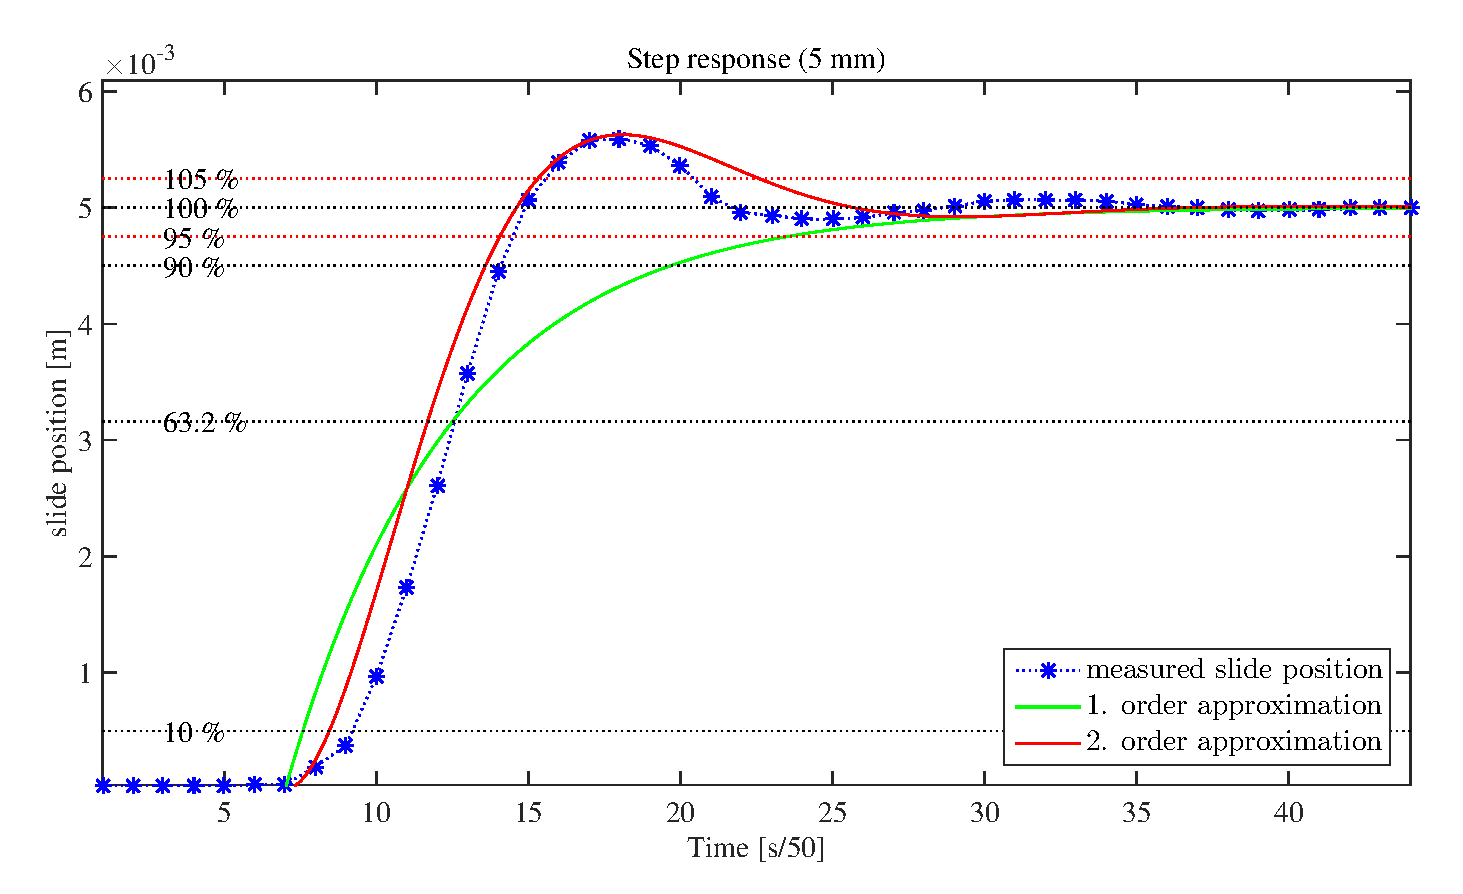
\includegraphics[scale=0.5]{step_slide.eps}
\caption{Step response from 0\,mm to 5\,mm. Plot details and measurements can be found in \autoref{app:cd} as \texttt{matlab\_scripts/slide\_step/plot\_slide\_pos.m}}. 
\label{fig:stepresponseslideapp}
\end{figure}
This completes this measurement log.